%% ++++++++++++++++++++++++++++++++++++++++++++++++++++++++++++
%% Hauptdatei, Wurzel des Dokuments
%% ++++++++++++++++++++++++++++++++++++++++++++++++++++++++++++
%
%  Gerüst:
%  * Version 0.11
%  * Dipl.-Ing. Karsten Renhak, karsten.renhak@tu-ilmenau.de
%  * Fachgebiet Kommunikationsnetze, TU Ilmenau
%
%  Für Hauptseminare, Studienarbeiten, Diplomarbeiten
%
%  Autor           : Max Mustermann
%  Letzte Änderung : 31.12.2011
%

% Headerfeld, Typ des Dokumentes, einzubindende Packages.
% Hier bei Bedarf Änderungen vornehmen.
\documentclass
[   twoside=false,     % Einseitiger oder zweiseitiger Druck?
    fontsize=11pt,     % Bezug: 12-Punkt Schriftgröße
    %DIV=15,            % Randaufteilung, siehe Dokumentation "KOMA"-Script
    %BCOR=17mm,         % Bindekorrektur: Innen 17mm Platz lassen. Copyshop-getestet
    headsepline,  % Unter Kopfzeile Trennlinie (aus: headnosepline)
    footsepline,  % Über Fußzeile Trennlinie (aus: footnosepline)
    open=right,        % Neue Kapitel im zweiseitigen Druck rechts beginnen lassen
    paper=a4,          % Seitenformat A4
    abstract=false,     % Abstract einbinden
    listof=totoc,      % Div. Verzeichnisse ins Inhaltsverzeichnis aufnehmen
    bibliography=totoc,% Literaturverzeichnis ins Inhaltsverzeichnis aufnehmen
    titlepage,         % Titelseite aktivieren
    headinclude=true,  % Seiten-Head in die Satzspiegelberechnung mit einbeziehen
    footinclude=false, % Seiten-Foot nicht in die Satzspiegelberechnung mit einbeziehen
    numbers=noenddot   % Gliederungsnummern ohne abschließenden Punkt darstellen
]   {scrreprt}         % Dokumentenstil: "Report" aus dem KOMA-Skript-Paket

\usepackage[active]{srcltx}
%\usepackage[activate=normal]{pdfcprot} % Optischer Randausgleich -> pdflatex!
\usepackage{ifthen}
\usepackage[german]{babel}
%\usepackage[latin1]{inputenc} % Zeichencodierung nach ISO-8859-1
\usepackage[utf8]{inputenc}   %	Zeichencodierung nach UTF-8 (Unicode)
\usepackage[T1]{fontenc}
%\usepackage{ae} % obsolet und durch lmodern ersetzt
\usepackage{lmodern}
\usepackage[T1]{url}
\usepackage[final]{graphicx}
\usepackage[automark]{scrpage2}
\usepackage{setspace}
%\usepackage[first,light]{draftcopy} % Für Probedruck
\usepackage[plainpages=false,pdfpagelabels,hypertexnames=false]{hyperref}
%Listing-Settings
\usepackage{listings}
\usepackage{courier}
\lstset{basicstyle=\footnotesize\ttfamily,breaklines=true}
% Nomencl-settings
\usepackage[intoc]{nomencl}
\AtBeginDocument{\setlength{\nomlabelwidth}{.4\columnwidth}}
\let\abbrev\nomenclature
\renewcommand{\nomname}{Abkürzungs- und Akronymverzeichnis}
\renewcommand{\nomlabel}[1]{#1 \dotfill}
\setlength{\nomitemsep}{-\parsep}
\makenomenclature
% Package für Tabellen
\usepackage{tabularx}
% Package 2 für Tabellen
\usepackage{longtable}
\usepackage{ragged2e,array,longtable}
% Linienstärkenfix für Tabellen
\setlength\arrayrulewidth{1pt}
% Package für Haken & Farbe
\usepackage{amssymb}
\usepackage[fleqn]{amsmath} % For creating equations without numbers
%\usepackage{color}
\usepackage[xcdraw]{xcolor}
%Package für Eurozeichen
\usepackage{eurosym}
%Package für Querformatmodus
\usepackage{lscape}
%Package for making dirtrees
\usepackage{dirtree}

\usepackage{enumitem}
\newcommand\CMSF[1]{\textcolor{orange}{SF: #1}} % For comments
\setlist[enumerate]{leftmargin=15pt}

% Definitions for Listings
\colorlet{punct}{red!60!black}
\definecolor{background}{HTML}{EEEEEE}
\definecolor{delim}{RGB}{20,105,176}
\colorlet{numb}{magenta!60!black}

\lstdefinelanguage{json}{
	basicstyle=\normalfont\ttfamily,
	numbers=left,
	numberstyle=\scriptsize,
	stepnumber=1,
	numbersep=8pt,
	showstringspaces=false,
	breaklines=true,
	frame=lines,
	backgroundcolor=\color{background},
	literate=
	*{0}{{{\color{numb}0}}}{1}
	{1}{{{\color{numb}1}}}{1}
	{2}{{{\color{numb}2}}}{1}
	{3}{{{\color{numb}3}}}{1}
	{4}{{{\color{numb}4}}}{1}
	{5}{{{\color{numb}5}}}{1}
	{6}{{{\color{numb}6}}}{1}
	{7}{{{\color{numb}7}}}{1}
	{8}{{{\color{numb}8}}}{1}
	{9}{{{\color{numb}9}}}{1}
	{:}{{{\color{punct}{:}}}}{1}
	{,}{{{\color{punct}{,}}}}{1}
	{\{}{{{\color{delim}{\{}}}}{1}
	{\}}{{{\color{delim}{\}}}}}{1}
	{[}{{{\color{delim}{[}}}}{1}
	{]}{{{\color{delim}{]}}}}{1},
}



% \usepackage{float}
% Package for defining new floats
\usepackage{newfloat}
% Define myequation as new float environment
\DeclareFloatingEnvironment[fileext=lop]{Equation}

\usepackage{microtype}
%Paket für Seitenränder
\usepackage{geometry}
\usepackage{colortbl}
\usepackage{pdfpages}
\usepackage{verbatim} %Block Comments
\usepackage{spverbatim} %Block Code with line break
\geometry{a4paper, top=30mm, left=40mm, right=30mm, bottom=30mm}

% For drawing numbers with circles around
\usepackage{tikz}
\newcommand*\circled[1]{\tikz[baseline=(char.base)]{
		\node[shape=circle,draw,inner sep=2pt] (char) {#1};}}

% Tiefe der Kapitelnummerierung beeinflussen
\setcounter{secnumdepth}{2} % Tiefe der Nummerierung
\setcounter{tocdepth}{2}    % Tiefe des Inhaltsverzeichnisses

% Hier in die zweite geschweifte Klammer jeweils
% die persönlichen Daten und das Thema der Arbeit eintragen:
\newcommand{\artderausarbeitung}{Hauptseminar}
\newcommand{\namedesautors}{}
\newcommand{\themaderarbeit}{Thema der Arbeit}
%\renewcommand*{\chapterheadstartvskip}{\vspace*{.1\baselineskip}}
\renewcommand*\chapterheadstartvskip{\vspace*{-\topskip}}
\renewcommand*{\chapterheadendvskip}{\vspace*{1.5\baselineskip}}

% PDF Metadaten definieren
\hypersetup{
   pdftitle={\themaderarbeit},
   pdfsubject={\artderausarbeitung},
   pdfauthor={\namedesautors},
   pdfkeywords={\artderausarbeitung Hauptseminar}}


% Abkürzungsverzeichnis beeinflussen. Hier nichts ändern!
\usepackage{acronym}

% Seitenlayout festlegen. Hier nichts ändern!
\pagestyle{scrplain}
\ihead[]{\headmark}
\ohead[]{}
\chead[]{}
\ifoot[]{}
\ofoot[]{}
\cfoot[]{\pagemark}
\renewcommand{\titlepagestyle}{scrheadings}
\renewcommand{\partpagestyle}{scrheadings}
\renewcommand{\chapterpagestyle}{scrheadings}
\renewcommand{\indexpagestyle}{scrheadings}

% Abschnittsweise Nummerierung anstatt fortlaufend. Hier nichts ändern!
\makeatletter
\@addtoreset{equation}{chapter}
\@addtoreset{figure}{chapter}
\@addtoreset{table}{chapter}
\renewcommand\theequation{\thechapter.\@arabic\c@equation}
\renewcommand\thefigure{\thechapter.\@arabic\c@figure}
\renewcommand\thetable{\thechapter.\@arabic\c@table}
\makeatother

% Quelltextrahmen, klein. Hier nichts ändern!
\newsavebox{\inhaltkl}
\def\rahmenkl{\sbox{\inhaltkl}\bgroup\small\renewcommand{\baselinestretch}{1}\vbox\bgroup\hsize\textwidth}
\def\endrahmenkl{\par\vskip-\lastskip\egroup\egroup\fboxsep3mm%
\framebox[\textwidth][l]{\usebox{\inhaltkl}}}

% Quelltextrahmen, normale Groesse. Hier nichts ändern!
\newsavebox{\inhalt}
\def\rahmen{\sbox{\inhalt}\bgroup\renewcommand{\baselinestretch}{1}\vbox\bgroup\hsize\textwidth}
\def\endrahmen{\par\vskip-\lastskip\egroup\egroup\fboxsep3mm%
\framebox[\textwidth][l]{\usebox{\inhalt}}}

% Trennvorschläge für falsch getrennte Wörter.
% Wird häufig bei eingedeutschen Wörtern benötigt, da LaTeX hierbei
% gerne falsch trennt. Alternativ kann auch im Fliesstext ein
% Trennvorschlag per "\-" hinterlegt werden, bspw.:
% Die Hard\-ware besteht aus A und B.
\hyphenation{
Hard-ware
}

% Sonstige Befehlsdefinitionen hier ablegen.
\newcommand{\entspricht}{\stackrel{\wedge}{=}}

% Tabellenspaltendefinitionen mit fester Breite --> somit Zeilenumbruch innerhalb einer Zelle möglich
% aus http://www.torsten-schuetze.de/tex/tabsatz-2004.pdf
\usepackage{array, booktabs}
\newcolumntype{f}{>{$}l<{$}}
\newcolumntype{n}{>{\raggedright}l}
\newcolumntype{N}{>{\scriptsize}l}
\newcolumntype{v}[1]{>{\raggedright\hspace{0pt}}m{#1}}
\newcolumntype{V}[1]{>{\scriptsize\raggedright\hspace{0pt}}m{#1}}
\newcolumntype{Z}[1]{>{\raggedright\centering}m{#1}}
\newcolumntype{k}[1]{>{\raggedright}p{#1}}
% ergibt Tabllenspalte fester Breite, linksbündig
% Umbruch innerhalb der Zelle mit \\, neue Tabellezeile mit \tabularnewline
% \addlinespace für Gruppentrennung (aus \texttt{booktabs.sty})
\usepackage{url} % Package for URL line breaks in bibliography
\def\UrlBreaks{\do\/\do-}

\begin{document}
\begin{spacing}{1,5}
%% ++++++++++++++++++++++++++++++++++++++++++++++++++++++++++++
%% Titelblatt
%% ++++++++++++++++++++++++++++++++++++++++++++++++++++++++++++
%
%  Gerüst:
%  * Version 0.11
%  * Dipl.-Ing. Karsten Renhak, karsten.renhak@tu-ilmenau.de
%  * Fachgebiet Kommunikationsnetze, TU Ilmenau
%
%  Für Hauptseminare, Studienarbeiten, Diplomarbeiten
%
%  Autor           : Max Mustermann
%  Letzte Änderung : 31.12.2011
%

\begin{titlepage}
	\centering
	
\includegraphics[scale=0.5]{images/logo}\\[3ex]
	{\Large \textsc{Technische Universität Ilmenau}}\\[3ex]
	{\Large Fakultät für Elektrotechnik und Informationstechnik}\\[3ex]
	\vfill
	{\Large \textbf{\artderausarbeitung}}\\[4ex]
	{\large \textbf{\themaderarbeit}}\\[4ex]
	\vfill
	\begin{tabular}{rl}
		\hline\\
		Eingereicht von:          & \quad Max\\[1.5ex]
								  & \quad Mustermann (Matrikelnr.: 12345)\\[1,5ex]
		Eingereicht am:         & \quad \today\\[1,5ex]
		Studiengang:            & \quad Medientechnologie\\[1,5ex]
		Fachgebiet:
		& \quad Audiovisuelle Technik\\[1,5ex]
		& \quad Institut für Medientechnik\\[1,5ex]
		%& \quad Department of Electrical Engineering\\[1,5ex]
		%& \quad and Information Technology\\[1,5ex]
		Betreuender Professor:
		& \quad Prof. Dr.-Ing. Alexander Raake \\[1,5ex]
		Wissenschaftlicher Betreuer:
		& \quad M.Sc. Stephan Fremerey
	\end{tabular}
	\vfill
\end{titlepage}


% Danksagung + Abstract einbinden
% \cleardoublepage
\noindent {\Large \textbf{Acknowledgments}}\\[4ex]
Firstly, I want to thank my Professor Prof. Dr.-Ing. Alexander Raake and academic advisor M.Sc. Ashutosh Singla for supervising my thesis and all the fruitful discussions during this work. Furthermore, I want to thank the staff of the media lab for the technical support of my thesis. I also want to thank all the persons participating in my proof of concept test, my family and friends and Mr. Dipl.-Ing. Karsten Renhak of Communication Networks Group at TU Ilmenau for publishing this LaTeX-template.

% Kann entfernt werden wenn mit Hauptteil begonnen
\cleardoublepage
\pagenumbering{roman} % Nummerierung der Seiten ab hier: 1, 2, 3, 4...
\pagestyle{scrheadings}


% Inhaltsverzeichnis
\cleardoublepage % Seitenumbruch erzwingen vor Änderung des Nummerierungsstils
%\pagenumbering{roman} % Nummerierung der Seiten ab hier: i, ii, iii, iv...
\pagestyle{scrheadings} % Ab hier mit Kopf- und Fusszeile
\tableofcontents
% Die einzelnen Kapitel
\cleardoublepage % Seitenumbruch erzwingen vor Änderung des Nummerierungsstils
\pagenumbering{arabic} % Nummerierung der Seiten ab hier: 1, 2, 3, 4...
%\cleardoublepage
\ihead[]{Abstract}
\chapter*{Abstract}
\addcontentsline{toc}{chapter}{Abstract}
\begin{spacing}{1.1}
Some text here.
\end{spacing}
\chapter{Einleitung}
\ihead[]{Einleitung}
\begin{spacing}{1.1}
	
\noindent Das ist ein Demozitat. (vgl. \cite{link:oculus_headtracking_sensors}) Die Mathematikumgebung kann in \LaTeX\ ebenfalls verwendet werden: $1+1=2$ oder 360$^{\circ}$.
Es können auch Fußnoten gesetzt werden: \texttt{Tabel}\footnote{https://tabel.withgoogle.com} ist ein Projekt von Google. \\ \\
Im Folgenden wird beim Zitat auch der Verweis zur jeweiligen Seite angezeigt: \cite[S. 1]{book:gibson1986ecological} oder \cite[S. 2-4]{corbillon2016viewport}. \\
Nun wird eine neue Seite begonnen. \newpage

\section{Unterkapitel}
\label{sec:unterkapitel1}
Im Folgenden wird eine Abbildung eingebunden:
\begin{figure}[!h]
	\centering
	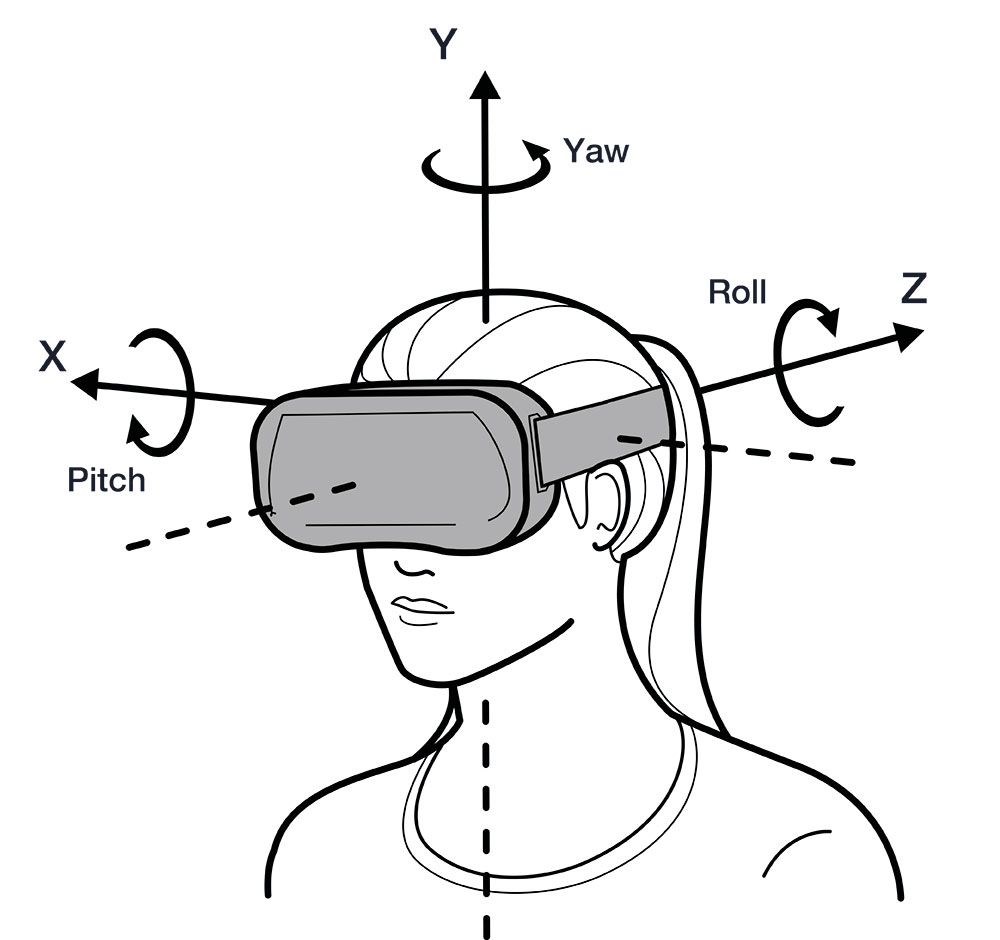
\includegraphics[width=7cm]{images/pyr_coordinates.jpg}
	\caption{Pitch Yaw Roll Koordinaten \cite{link:oculus_headtracking_sensors}}
	\label{picture:pyr_coordinates}
\end{figure}

\noindent Kapitel, Abbildungen etc. können auch mittels Verwendung des jeweiligen Labels referenziert werden. Z.B.: Siehe Kapitel \ref{sec:unterkapitel1}. In Abbildung \ref{picture:pyr_coordinates} sind die verschiedenen Winkelmaße dargestellt, die z.B. Kopfrotationsdaten beschreiben können. \\
Aufzählungen sehen so aus:
\begin{itemize}
	\setlength\itemsep{0.1em}
	\item Aufzählungspunkt 1
	\item Aufzählungspunkt 2
	\item ...
\end{itemize}
Abkürzungen werden zuerst ins Abkürzungsverzeichnis eingetragen und können dann aufgerufen werden: \ac{JPEG}. Bei späterer Erwähnung der Abkürzung \ac{JPEG} wird die definierte Kurzform übernommen.

\subsection{Unterunterkapitel}
Im Folgenden ist Tabelle \ref{table:factors_and_descriptions} dargestellt. Diese können auch direkt mit \LaTeX\ erstellt werden.
\begin{table}[!h]
	\begin{tabular}{|p{2.7cm}|p{10.5cm}|}\hline
		\rowcolor[gray] {.6} \textbf{Faktor} & \textbf{Beschreibung} \\ \hline
		
		\rowcolor[gray] {.8} \multicolumn{2}{|l|}{\textbf{Unterüberschrift 1}} \\ \hline
		Faktor 1 & Beschreibung 1 \\ \hline
		Faktor 2 & Beschreibung 2 \\ \hline
		\rowcolor[gray] {.8} \multicolumn{2}{|l|}{\textbf{Unterüberschrift 2}} \\ \hline
		Faktor 3 & Beschreibung 3 \\ \hline
		Faktor 4 & Beschreibung 4 \\ \hline
	\end{tabular}
	\caption{Faktoren mit Beschreibung}
	\label{table:factors_and_descriptions}
\end{table}

\end{spacing}
\chapter{Hauptkapitel}
\ihead[]{Hauptkapitel}
\begin{spacing}{1.1}
Hier ist Platz für etwas Text.
\end{spacing}

\chapter{Fazit und Ausblick}
\ihead[]{Fazit und Ausblick}
\begin{spacing}{1.1}
	Hier ist Platz für etwas Text.
\end{spacing}
\cleardoublepage
\ihead[]{Literaturverzeichnis}
%\chapter{}
\ihead[]{}
\begin{spacing}{1.1}
Hier ist Platz für etwas Text.
\end{spacing}
%\chapter{Fazit und Ausblick}
\ihead[]{Fazit und Ausblick}
\begin{spacing}{1.1}
Hier ist Platz für etwas Text.
\end{spacing}

\appendix

% Literaturverzeichnis einbinden
%% ++++++++++++++++++++++++++++++++++++++++++++++++++++++++++++
%% Anhang: Literaturverzeichnis
%% ++++++++++++++++++++++++++++++++++++++++++++++++++++++++++++
%
%  Gerüst:
%  * Version 0.11
%  * Dipl.-Ing. Karsten Renhak, karsten.renhak@tu-ilmenau.de
%  * Fachgebiet Kommunikationsnetze, TU Ilmenau
%
%  Für Hauptseminare, Studienarbeiten, Diplomarbeiten
%
%  Autor           : Max Mustermann
%  Letzte Änderung : 31.12.2011
%

% Mit dem Befehl \nocite werden auch nicht im Text zitierte
% aus der Literaturdatenbank mit in das Literaturverzeichnis aufgenommen.
% Ein "\nocite{*}" übernimmt ungeprüft die komplette Datenbank.
%\nocite{*}
\begin{spacing}{1.1}
\ihead[]{Literaturverzeichnis}
\bibliographystyle{plaindin}
\bibliography{bibliography_books,bibliography_paper,bibliography_miscellaneous,bibliography_weblinks}
\end{spacing}
% Alternativ: Mehrere Datenbanken verwenden, falls eine
% oder mehrere umfangreiche Sammlungen exisitieren:
%\bibliography{literatur_buecher,literatur_weblinks}

% Abkürzungsverzeichnis einbinden
%% ++++++++++++++++++++++++++++++++++++++++++++++++++++++++++++
%% Anhang: Abkürzungsverzeichnis
%% ++++++++++++++++++++++++++++++++++++++++++++++++++++++++++++
%
%  Gerüst:
%  * Version 0.11
%  * Dipl.-Ing. Karsten Renhak, karsten.renhak@tu-ilmenau.de
%  * Fachgebiet Kommunikationsnetze, TU Ilmenau
%
%  Für Hauptseminare, Studienarbeiten, Diplomarbeiten
%
%  Autor           : Max Mustermann
%  Letzte Änderung : 31.12.2011
%

% Hier keine weiteren Änderungen vornehmen
%\chapter*{Abbreviations- and acronyms directory}
%\addcontentsline{toc}{chapter}{Abbreviations- and acronyms directory}
\cleardoublepage
\ihead[]{Abkürzungs- und Akronymverzeichnis}
\chapter*{Abkürzungs- und Akronymverzeichnis}
\addcontentsline{toc}{chapter}{Abkürzungs- und Akronymverzeichnis}
\begin{spacing}{1.1}
\begin{acronym}[XXXXXXXXX]
	\acro{ACMMM}{Association for Computing Machinery Multimedia}
	\acro{AMOLED}{Active-matrix Organic Light-emitting Diode}
	\acro{JPEG}{Joint Photographic Experts Group}
\end{acronym}
\end{spacing}

% Abbildungsverzeichnis einbinden
\cleardoublepage
\ihead[]{Abbildungsverzeichnis}
\listoffigures

% Tabellenverzeichnis einbinden
%%% ++++++++++++++++++++++++++++++++++++++++++++++++++++++++++++
%% Anhang: Tabellenverzeichnis
%% ++++++++++++++++++++++++++++++++++++++++++++++++++++++++++++
%
%  Gerüst:
%  * Version 0.11
%  * Dipl.-Ing. Karsten Renhak, karsten.renhak@tu-ilmenau.de
%  * Fachgebiet Kommunikationsnetze, TU Ilmenau
%
%  Für Hauptseminare, Studienarbeiten, Diplomarbeiten
%
%  Autor           : Max Mustermann
%  Letzte Änderung : 31.12.2011
%

% Hier keine weiteren Änderungen vornehmen
\cleardoublepage
\ihead[]{List of Tables}
\listoftables

% Anhang einbinden
%\renewcommand{\thesection}{\Alph{section}}
%\chapter[Appendix]{Appendix}
%\contentsname{\def\chaptername{Appendix}}
\ihead[]{Appendix}
%\addcontentsline{toc}{chapter}{Appendix}

\section{Simulator Sickness Questionnaire} \label{appendix:SSQ}

\begin{table}[!h]
	\centering
	\begin{tabular}{|c|c|c|c|}\hline
		\rowcolor[gray] {.6} \textbf{SSQ Symptom\footnotemark} & \textbf{N} & \textbf{O} & \textbf{D} \\ \hline
		General discomfort & 1 & 1 &  \\ \hline
		Fatigue &  & 1 &  \\ \hline
		Headache &  & 1 &  \\ \hline
		Eyestrain &  & 1 &  \\ \hline
		Difficulty focusing &  & 1 & 1 \\ \hline
		Increased salivation & 1 &  &  \\ \hline
		Sweating & 1 &  &  \\ \hline
		Nausea & 1 &  & 1 \\ \hline
		Difficulty concentrating & 1 & 1 &  \\ \hline
		Fullness of head &  &  & 1 \\ \hline
		Blurred vision &  & 1 & 1 \\ \hline
		Dizzy (eyes open) &  &  & 1 \\ \hline
		Dizzy (eyes closed) &  &  & 1 \\ \hline
		Vertigo &  &  & 1 \\ \hline
		Stomach awareness & 1 &  &  \\ \hline
		Burping & 1 &  &  \\ \hline \hline
		Total\footnotemark & [1] & [2] & [3] \\ \hline
	\end{tabular}
	\caption{SSQ symptoms and related weights (cf. \cite[p. 212]{kennedy1993simulator})}
	\label{table:SSQ_symptoms_weights}
\end{table}
\noindent Calculation of scores according to \cite[p. 212]{kennedy1993simulator}: \\
$N=[1]*9.54$\\
$O=[2]*7.58$\\
$D=[3]*13.92$\\
$TS=([1]+[2]+[3])*3.74$
\footnotetext[1]{Scored 0, 1, 2, 3.}
\footnotetext[2]{Sum calculated by adding symptom scores. All omitted scores in the table are zero.}
\newpage

\section{Technical specifications of HTC Vive and Oculus Rift} \label{appendix:vive_rift_specs}


\begin{table}[!h]
	\centering
	\begin{tabular}{|p{2.8cm}|p{4.8cm}|p{4.8cm}|}\hline
		\rowcolor[gray] {.6} \textbf{Parameter} & \textbf{HTC Vive} & \textbf{Oculus Rift} \\ \hline
		Display & OLED & OLED \\ \hline
		Resolution & $2160 \times 1200$ & $2160 \times 1200$ \\ \hline
		Display Refresh rate & 90\,Hz & 90\,Hz \\ \hline
		Display Pixel density (cf. \cite{link:tomshardware_vive_rift_specs}) & 447\,ppi & 456\,ppi \\ \hline
		Field of View & $110^{\circ}$ & $110^{\circ}$ \\ \hline
		Sensors & Accelerometer, gyroscope, magnetometer, constellation tracking camera & Accelerometer, gyroscope, Lighthouse tracking system, front-facing camera \\ \hline
		Connections & HDMI, USB 2.0, USB 3.0 & HDMI, USB 2.0, USB 3.0 \\ \hline
	\end{tabular}
	\caption{Specifications of HTC Vive and Oculus Rift (cf.  \cite{link:tomshardware_vive_rift_specs}, \cite{link:rift_vive_specs_digitaltrends}, \cite{link:vive_homepage})}
	\label{table:specs_vive_rift}
\end{table}

\section{Technical specifications of Merge VR} \label{appendix:mergevr_specs}

\begin{table}[!h]
	\centering
	\begin{tabular}{|p{2.8cm}|p{6cm}|}\hline
		\rowcolor[gray] {.6} \textbf{Parameter} & \textbf{Merge VR} \\ \hline
		Field of View & $96^{\circ}$ \\ \hline
		Lens diameter & 42\,mm \\ \hline
		Display & Dependent on inserted device \\ \hline
		Resolution & Dependent on inserted device \\ \hline
		Display Refresh rate & Dependent on inserted device \\ \hline
		Sensors & Dependent on inserted device \\ \hline
	\end{tabular}
	\caption{Specifications of Merge VR (cf. \cite{link:mergevr_goggles})}
	\label{table:mergevr_specs}
\end{table}


\section{Technical Specifications of Qualisys PC} \label{appendix:qualisys_specs}
\begin{table}[!h]
	\centering
	\begin{tabular}{|>{\RaggedRight}p{3cm}|>{\RaggedRight}p{9cm}|}\hline
		\rowcolor[gray] {.6} \textbf{Component} & \textbf{Name} \\ \hline
		CPU & Intel Core i7-6700K \\ \hline
		Graphics card & NVIDIA GeForce GTX 750 Ti \\ \hline
		RAM & 16\,GB \\ \hline
		Network adapter & Intel I211 Ethernet Controller \\ \hline
		Harddisk & Samsung SSD 750 Evo 250\,GB,\newline WDC WD20EFRX-68EUZN0 \\ \hline
		OS & Windows 10 \\ \hline
	\end{tabular}
	\caption{Technical specifications of Qualisys PC}
\end{table}


\section{Technical Specifications of lab PC} \label{appendix:specs_lab_pc}
\begin{table}[!h]
	\centering
	\begin{tabular}{|>{\RaggedRight}p{3cm}|>{\RaggedRight}p{9cm}|}\hline
		\rowcolor[gray] {.6} \textbf{Component} & \textbf{Name} \\ \hline
		CPU & Intel Core i7-6700K \\ \hline
		Graphics card & NVIDIA GeForce GTX 980 Ti \\ \hline
		RAM & 16\,GB \\ \hline
		Network adapter & Intel I219-V Ethernet Controller \\ \hline
		Harddisk & Samsung SSD 850 Evo 500\,GB,\newline WDC WD1003FZEX-00MK2A0 \\ \hline
		OS & Windows 7 \\ \hline
	\end{tabular}
	\caption{Technical specifications of lab PC}
\end{table}


\section{Technical Specifications of Motorola Moto Z} \label{appendix:specs_moto_z}
\begin{table}[!h]
	\centering
	\begin{tabular}{|>{\RaggedRight}p{3cm}|>{\RaggedRight}p{9cm}|}\hline
		\rowcolor[gray] {.6} \textbf{Component} & \textbf{Name} \\ \hline
		Chipset & Qualcomm MSM8996 Snapdragon 820 \\ \hline
		GPU & Adreno 530 \\ \hline
		RAM & 4\,GB \\ \hline
		Memory & 32\,GB internal \\ \hline
		Display & 5.5\,'' $1440\times2560$ AMOLED screen ($\approx535\,ppi$) \\ \hline
		Sensors & Fingerprint, accelerometer, gyroscope, proximity, compass \\ \hline
		OS & Android 7.0 \\ \hline
	\end{tabular}
	\caption{Technical specifications of Motorola Moto Z (cf. \cite{link:moto_z_specs})}
\end{table}

\section{Additional Information about Test Sequences} \label{appendix:additional_information_sequences}
\begin{table}[!h]
	\centering
	\begin{tabular}{|p{0.5cm}|p{3.2cm}|p{8.7cm}|}\hline
		\rowcolor[gray] {.6} \textbf{ID} & \textbf{Timestamp} & \textbf{Link} \\ \hline
		1 & 00:00:08 – 00:03:01 & / (student project) \\ \hline
		2 & 00:00:22 – 00:03:01 & https://www.youtube.com/watch?v=yA34HDry2P8 \\ \hline
		3 & 00:00:03 – 00:03:01 & https://www.youtube.com/watch?v=jU-pZSsYhDk \\ \hline
	\end{tabular}
	\caption{Timestamps and links of used test sequences}
\end{table}

\begin{figure}[!h]
	\centering
	\includegraphics[width=10cm]{pictures/SITI_1.pdf}
	\caption{SI/TI values per frame of sequence 1 (source: own figure)}
	\label{picture:siti_1}
\end{figure}

\begin{figure}[!h]
	\centering
	\includegraphics[width=10cm]{pictures/SITI_2.pdf}
	\caption{SI/TI values per frame of sequence 2 (source: own figure)}
	\label{picture:siti_2}
\end{figure}

\begin{figure}[!h]
	\centering
	\includegraphics[width=10cm]{pictures/SITI_3.pdf}
	\caption{SI/TI values per frame of sequence 3 (source: own figure)}
	\label{picture:siti_3}
\end{figure}

\cleardoublepage

\section{Questionnaires used in Proof of Concept Test} \label{appendix:questionnaires}
\begin{figure}[!h]
	\centering
	\includegraphics[width=14cm]{pictures/poc_questionnairesp1.pdf}
	\caption{Page 1 of questionnaires used in the PoC test (source: own figure)}
	\label{picture:poc_questionnairesp1}
\end{figure}

\cleardoublepage

\begin{figure}[!h]
	\centering
	\includegraphics[width=14cm]{pictures/poc_questionnairesp2-4.pdf}
	\caption{Page 2-4 of questionnaires used in the PoC test (source: own figure)}
	\label{picture:poc_questionnairesp2-4}
\end{figure}


\section{Parameters of \textit{headify\_shift\_cut\_merge.py}} \label{appendix:headify_shiftcutmerge}

\begin{table}[!h]
	\centering
	\begin{tabular}{|>{\RaggedRight}p{3cm}|>{\RaggedRight}p{10cm}|}\hline
		\rowcolor[gray] {.6} \textbf{Parameter} & \textbf{Feature} \\ \hline
		-cut & Enable synchronisation between Qualisys data and external device by cutting off the not relevant parts of the video.
		 \\ \hline
		 -h & Add this parameter to display the help. \\ \hline
		-onlymerge & Only merge the datasets located in the \textit{data\_modified} directory, hence neither shift or cut them.
		 \\ \hline
		-subjects & The number of datasets to evaluate. \\ \hline
		-yawvalues & The name of the JSON file containing the measured yaw values in the standard position per subject and HMD.
		 \\ \hline
	\end{tabular}
	\caption{Command line parameters of \textit{headify\_shift\_cut\_merge.py}}
	\label{table:headify_shiftcutmerge}
\end{table}


\section{Parameters of \textit{headify\_evaluation.py}} \label{appendix:headify_evaluation}

\begin{table}[!h]
	\centering
	\begin{tabular}{|>{\RaggedRight}p{3cm}|>{\RaggedRight}p{10cm}|}\hline
		\rowcolor[gray] {.6} \textbf{Parameter} & \textbf{Feature} \\ \hline
		-dynamicfov & The integer percentage value of the dynamic FoV to calculate. \\ \hline
		-euclideandist & Plot the mean euclidean distance between Qualisys and the used HMD. \\ \hline
		-fovvideos & Renders videos showing single FoV per subject and dynamic calculated mean FoV including XX\% of all subjects FoVs (adaptable via -dynamicfov). \\ \hline
		-headturns & Plots mean number of head turns per subject, mean number of head turns per video and HMD and mean number of head turns for videos watched for the first and second time, irrespective of the used HMD.  \\ \hline
		-plotdynamicfov & Plot the dynamic FoV over time and the mean. \\ \hline
		-qualisys & Enable evaluation of data recorded by Qualisys. \\ \hline
		-singlevideos & Plot recorded head rotations over time. If Qualisys parameter enabled, the euclidean distance between both curves will be plot. \\ \hline
		-standby & Send PC to standby after calculations. \\ \hline
		-shutdown & Shut down PC after calculations. \\ \hline
	\end{tabular}
	\caption{Command line parameters of \textit{headify\_evaluation.py}}
	\label{table:commands_headify_evaluation}
\end{table}


% Eigenständigkeitserklärung
\cleardoublepage
\ihead[]{Eigenständigkeitserklärung}
\chapter*{Eigenständigkeitserklärung}
\addcontentsline{toc}{chapter}{Eigenständigkeitserklärung}
\begin{spacing}{1.1}
Hiermit erkläre ich, dass ich diese Arbeit selbstständig durchgeführt und abgefasst habe. Quellen, Literatur und Hilfsmittel, die von mir genutzt wurden, sind als solche
gekennzeichnet.
\\[2cm]
\end{spacing}
\noindent Ilmenau, den \today\hfill
\\[2cm]
\parbox{4cm}{\centering \hrule
	\strut \centering\footnotesize Max Mustermann}
\\[2cm]
    
\cleardoublepage

\end{spacing}
\end{document}
